% One step of the delivery robot (Section "An Agent Loop"): KRROOD, and what every build with a separate store has in common.
% Input inside a figure environment:  \centering% One step of the delivery robot (Section "An Agent Loop"): KRROOD, and what every build with a separate store has in common.
% Input inside a figure environment:  \centering% One step of the delivery robot (Section "An Agent Loop"): KRROOD, and what every build with a separate store has in common.
% Input inside a figure environment:  \centering% One step of the delivery robot (Section "An Agent Loop"): KRROOD, and what every build with a separate store has in common.
% Input inside a figure environment:  \centering\input{figures/agent_loop_builds.tex}
% Needs only \usepackage{tikz} in the preamble (no TikZ libraries); xcolor comes with acmart.
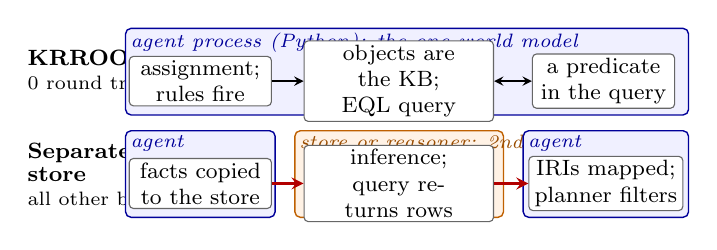
\begin{tikzpicture}[x=1cm, y=1cm, >=stealth, font=\footnotesize,
  agent/.style={draw=blue!60!black, fill=blue!6, rounded corners=2pt, line width=0.5pt},
  other/.style={draw=orange!75!black, fill=orange!10, rounded corners=2pt, line width=0.5pt},
  boxlabel/.style={font=\scriptsize\itshape, anchor=north west, inner sep=1.5pt},
  op/.style={draw=black!60, fill=white, rounded corners=1.5pt, align=center, inner sep=1.5pt,
    minimum height=0.62cm, font=\footnotesize},
  flow/.style={->, line width=0.5pt},
  cross/.style={->, line width=0.9pt, draw=red!70!black},
  rt/.style={circle, fill=red!70!black, text=white, inner sep=0pt, minimum size=8pt, font=\tiny\bfseries},
  rowname/.style={anchor=west, align=left, inner sep=0pt},
  head/.style={font=\scriptsize\bfseries, text=black!70},
]

% ---------------------------------------------------------------- KRROOD
\node[rowname] at (0,2.6) {\textbf{KRROOD}\\[-1pt]{\scriptsize 0 round trips}};
\draw[agent] (1.25,2.05) rectangle (8.4,3.15);
\node[boxlabel, text=blue!60!black] at (1.25,3.15) {agent process (Python): the one world model};
\node[op, text width=1.7cm] (k1) at (2.2,2.48) {assignment;\\rules fire};
\node[op, text width=2.3cm] (k2) at (4.72,2.48) {objects are the KB;\\EQL query};
\node[op, text width=1.7cm] (k3) at (7.32,2.48) {a predicate\\in the query};
\draw[flow] (k1) -- (k2);
\draw[flow, <->] (k2) -- (k3);

% ---------------------------------------------------------------- separate store
\node[rowname] at (0,1.3) {\textbf{Separate}\\[-1pt]\textbf{store}\\[-1pt]{\scriptsize all other builds}};
\draw[agent] (1.25,0.75) rectangle (3.15,1.85);
\node[boxlabel, text=blue!60!black] at (1.25,1.85) {agent};
\draw[other] (3.4,0.75) rectangle (6.05,1.85);
\node[boxlabel, text=orange!60!black] at (3.4,1.85) {store or reasoner: 2nd model};
\draw[agent] (6.3,0.75) rectangle (8.4,1.85);
\node[boxlabel, text=blue!60!black] at (6.3,1.85) {agent};
\node[op, text width=1.7cm] (g1) at (2.2,1.18) {facts copied\\to the store};
\node[op, text width=2.3cm] (g2) at (4.72,1.18) {inference;\\query returns rows};
\node[op, text width=1.85cm] (g3) at (7.35,1.18) {IRIs mapped;\\planner filters};
\draw[cross] (g1) -- (g2);
\draw[cross] (g2) -- (g3);
\end{tikzpicture}

% Needs only \usepackage{tikz} in the preamble (no TikZ libraries); xcolor comes with acmart.
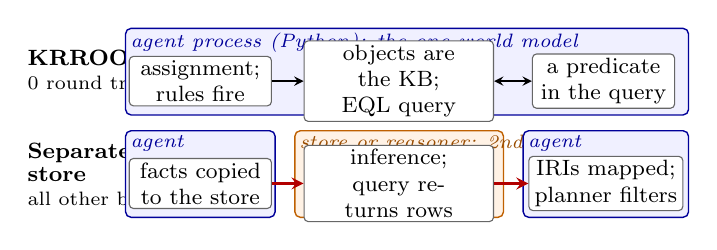
\begin{tikzpicture}[x=1cm, y=1cm, >=stealth, font=\footnotesize,
  agent/.style={draw=blue!60!black, fill=blue!6, rounded corners=2pt, line width=0.5pt},
  other/.style={draw=orange!75!black, fill=orange!10, rounded corners=2pt, line width=0.5pt},
  boxlabel/.style={font=\scriptsize\itshape, anchor=north west, inner sep=1.5pt},
  op/.style={draw=black!60, fill=white, rounded corners=1.5pt, align=center, inner sep=1.5pt,
    minimum height=0.62cm, font=\footnotesize},
  flow/.style={->, line width=0.5pt},
  cross/.style={->, line width=0.9pt, draw=red!70!black},
  rt/.style={circle, fill=red!70!black, text=white, inner sep=0pt, minimum size=8pt, font=\tiny\bfseries},
  rowname/.style={anchor=west, align=left, inner sep=0pt},
  head/.style={font=\scriptsize\bfseries, text=black!70},
]

% ---------------------------------------------------------------- KRROOD
\node[rowname] at (0,2.6) {\textbf{KRROOD}\\[-1pt]{\scriptsize 0 round trips}};
\draw[agent] (1.25,2.05) rectangle (8.4,3.15);
\node[boxlabel, text=blue!60!black] at (1.25,3.15) {agent process (Python): the one world model};
\node[op, text width=1.7cm] (k1) at (2.2,2.48) {assignment;\\rules fire};
\node[op, text width=2.3cm] (k2) at (4.72,2.48) {objects are the KB;\\EQL query};
\node[op, text width=1.7cm] (k3) at (7.32,2.48) {a predicate\\in the query};
\draw[flow] (k1) -- (k2);
\draw[flow, <->] (k2) -- (k3);

% ---------------------------------------------------------------- separate store
\node[rowname] at (0,1.3) {\textbf{Separate}\\[-1pt]\textbf{store}\\[-1pt]{\scriptsize all other builds}};
\draw[agent] (1.25,0.75) rectangle (3.15,1.85);
\node[boxlabel, text=blue!60!black] at (1.25,1.85) {agent};
\draw[other] (3.4,0.75) rectangle (6.05,1.85);
\node[boxlabel, text=orange!60!black] at (3.4,1.85) {store or reasoner: 2nd model};
\draw[agent] (6.3,0.75) rectangle (8.4,1.85);
\node[boxlabel, text=blue!60!black] at (6.3,1.85) {agent};
\node[op, text width=1.7cm] (g1) at (2.2,1.18) {facts copied\\to the store};
\node[op, text width=2.3cm] (g2) at (4.72,1.18) {inference;\\query returns rows};
\node[op, text width=1.85cm] (g3) at (7.35,1.18) {IRIs mapped;\\planner filters};
\draw[cross] (g1) -- (g2);
\draw[cross] (g2) -- (g3);
\end{tikzpicture}

% Needs only \usepackage{tikz} in the preamble (no TikZ libraries); xcolor comes with acmart.
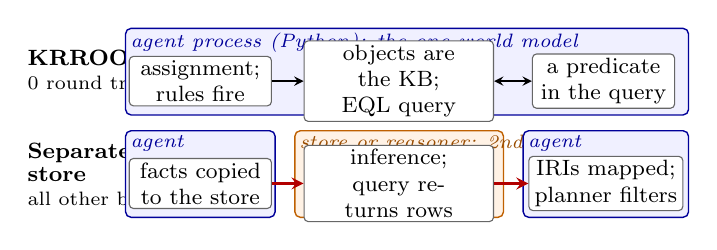
\begin{tikzpicture}[x=1cm, y=1cm, >=stealth, font=\footnotesize,
  agent/.style={draw=blue!60!black, fill=blue!6, rounded corners=2pt, line width=0.5pt},
  other/.style={draw=orange!75!black, fill=orange!10, rounded corners=2pt, line width=0.5pt},
  boxlabel/.style={font=\scriptsize\itshape, anchor=north west, inner sep=1.5pt},
  op/.style={draw=black!60, fill=white, rounded corners=1.5pt, align=center, inner sep=1.5pt,
    minimum height=0.62cm, font=\footnotesize},
  flow/.style={->, line width=0.5pt},
  cross/.style={->, line width=0.9pt, draw=red!70!black},
  rt/.style={circle, fill=red!70!black, text=white, inner sep=0pt, minimum size=8pt, font=\tiny\bfseries},
  rowname/.style={anchor=west, align=left, inner sep=0pt},
  head/.style={font=\scriptsize\bfseries, text=black!70},
]

% ---------------------------------------------------------------- KRROOD
\node[rowname] at (0,2.6) {\textbf{KRROOD}\\[-1pt]{\scriptsize 0 round trips}};
\draw[agent] (1.25,2.05) rectangle (8.4,3.15);
\node[boxlabel, text=blue!60!black] at (1.25,3.15) {agent process (Python): the one world model};
\node[op, text width=1.7cm] (k1) at (2.2,2.48) {assignment;\\rules fire};
\node[op, text width=2.3cm] (k2) at (4.72,2.48) {objects are the KB;\\EQL query};
\node[op, text width=1.7cm] (k3) at (7.32,2.48) {a predicate\\in the query};
\draw[flow] (k1) -- (k2);
\draw[flow, <->] (k2) -- (k3);

% ---------------------------------------------------------------- separate store
\node[rowname] at (0,1.3) {\textbf{Separate}\\[-1pt]\textbf{store}\\[-1pt]{\scriptsize all other builds}};
\draw[agent] (1.25,0.75) rectangle (3.15,1.85);
\node[boxlabel, text=blue!60!black] at (1.25,1.85) {agent};
\draw[other] (3.4,0.75) rectangle (6.05,1.85);
\node[boxlabel, text=orange!60!black] at (3.4,1.85) {store or reasoner: 2nd model};
\draw[agent] (6.3,0.75) rectangle (8.4,1.85);
\node[boxlabel, text=blue!60!black] at (6.3,1.85) {agent};
\node[op, text width=1.7cm] (g1) at (2.2,1.18) {facts copied\\to the store};
\node[op, text width=2.3cm] (g2) at (4.72,1.18) {inference;\\query returns rows};
\node[op, text width=1.85cm] (g3) at (7.35,1.18) {IRIs mapped;\\planner filters};
\draw[cross] (g1) -- (g2);
\draw[cross] (g2) -- (g3);
\end{tikzpicture}

% Needs only \usepackage{tikz} in the preamble (no TikZ libraries); xcolor comes with acmart.
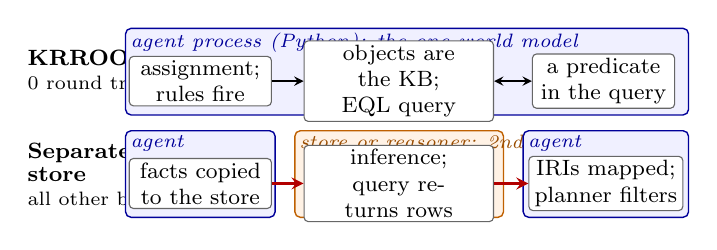
\begin{tikzpicture}[x=1cm, y=1cm, >=stealth, font=\footnotesize,
  agent/.style={draw=blue!60!black, fill=blue!6, rounded corners=2pt, line width=0.5pt},
  other/.style={draw=orange!75!black, fill=orange!10, rounded corners=2pt, line width=0.5pt},
  boxlabel/.style={font=\scriptsize\itshape, anchor=north west, inner sep=1.5pt},
  op/.style={draw=black!60, fill=white, rounded corners=1.5pt, align=center, inner sep=1.5pt,
    minimum height=0.62cm, font=\footnotesize},
  flow/.style={->, line width=0.5pt},
  cross/.style={->, line width=0.9pt, draw=red!70!black},
  rt/.style={circle, fill=red!70!black, text=white, inner sep=0pt, minimum size=8pt, font=\tiny\bfseries},
  rowname/.style={anchor=west, align=left, inner sep=0pt},
  head/.style={font=\scriptsize\bfseries, text=black!70},
]

% ---------------------------------------------------------------- KRROOD
\node[rowname] at (0,2.6) {\textbf{KRROOD}\\[-1pt]{\scriptsize 0 round trips}};
\draw[agent] (1.25,2.05) rectangle (8.4,3.15);
\node[boxlabel, text=blue!60!black] at (1.25,3.15) {agent process (Python): the one world model};
\node[op, text width=1.7cm] (k1) at (2.2,2.48) {assignment;\\rules fire};
\node[op, text width=2.3cm] (k2) at (4.72,2.48) {objects are the KB;\\EQL query};
\node[op, text width=1.7cm] (k3) at (7.32,2.48) {a predicate\\in the query};
\draw[flow] (k1) -- (k2);
\draw[flow, <->] (k2) -- (k3);

% ---------------------------------------------------------------- separate store
\node[rowname] at (0,1.3) {\textbf{Separate}\\[-1pt]\textbf{store}\\[-1pt]{\scriptsize all other builds}};
\draw[agent] (1.25,0.75) rectangle (3.15,1.85);
\node[boxlabel, text=blue!60!black] at (1.25,1.85) {agent};
\draw[other] (3.4,0.75) rectangle (6.05,1.85);
\node[boxlabel, text=orange!60!black] at (3.4,1.85) {store or reasoner: 2nd model};
\draw[agent] (6.3,0.75) rectangle (8.4,1.85);
\node[boxlabel, text=blue!60!black] at (6.3,1.85) {agent};
\node[op, text width=1.7cm] (g1) at (2.2,1.18) {facts copied\\to the store};
\node[op, text width=2.3cm] (g2) at (4.72,1.18) {inference;\\query returns rows};
\node[op, text width=1.85cm] (g3) at (7.35,1.18) {IRIs mapped;\\planner filters};
\draw[cross] (g1) -- (g2);
\draw[cross] (g2) -- (g3);
\end{tikzpicture}
